%%%%%%%%%%%%%%%%%%%%%%%%%%%%%%%%%%%%%%%%%%%%%%%%%%%%%%%%%%%%%%%%%%%%%
%  Emotion-Aware Image Caption Generation Report
%  Machine Learning Sessional
%  Team: TeamML Newbies
%%%%%%%%%%%%%%%%%%%%%%%%%%%%%%%%%%%%%%%%%%%%%%%%%%%%%%%%%%%%%%%%%%%%%

\documentclass[12pt]{article}

%%  PACKAGES
\usepackage[a4paper, top=1in, bottom=1in, left=1.1in, right=1.1in]{geometry}
\usepackage{setspace}
\usepackage[T1]{fontenc}
\usepackage[hidelinks, colorlinks=true, linkcolor=blue,
            citecolor=blue, urlcolor=blue]{hyperref}
\usepackage{graphicx}
\usepackage{booktabs}
\usepackage{amsmath}
\usepackage{amssymb}
\usepackage{float}
\usepackage{xcolor}
\usepackage{verbatim}
\usepackage{mdframed}
\usepackage{titlesec}
\usepackage{fancyhdr}
\usepackage{tikz}
\usepackage{subcaption}
\usepackage{multirow}
\usetikzlibrary{shapes,arrows,positioning,calc,fit,backgrounds,shadows}

\setlength{\headheight}{14.5pt}
\onehalfspacing

%%  COLORED BOX ENVIRONMENTS
\newmdenv[
  backgroundcolor=blue!6,
  linecolor=blue!60!black,
  linewidth=1.5pt,
  innertopmargin=6pt,
  innerbottommargin=6pt,
  skipabove=6pt,
  skipbelow=6pt
]{architecturebox}

\newmdenv[
  backgroundcolor=green!6,
  linecolor=green!50!black,
  linewidth=1.5pt,
  innertopmargin=6pt,
  innerbottommargin=6pt,
  skipabove=6pt,
  skipbelow=6pt
]{resultbox}

\newmdenv[
  backgroundcolor=orange!8,
  linecolor=orange!70!black,
  linewidth=1.5pt,
  innertopmargin=6pt,
  innerbottommargin=6pt,
  skipabove=6pt,
  skipbelow=6pt
]{deploymentbox}

\newmdenv[
  backgroundcolor=purple!6,
  linecolor=purple!60!black,
  linewidth=1.5pt,
  innertopmargin=6pt,
  innerbottommargin=6pt,
  skipabove=6pt,
  skipbelow=6pt
]{metricbox}

%%  PLACEHOLDER COMMAND FOR IMAGES
\newcommand{\imgplaceholder}[3]{%
  \begin{center}%
    \fbox{%
      \begin{minipage}{#1}%
        \vspace{#2}\par
        \centering
        \textcolor{gray}{\small\textit{[Image: #3]}}
        \vspace{#2}%
      \end{minipage}%
    }%
  \end{center}%
}

%%  SECTION FORMATTING
\titleformat{\section}{\Large\bfseries\color{blue!70!black}}{\thesection}{1em}{}[\titlerule]
\titleformat{\subsection}{\large\bfseries\color{blue!60!black}}{\thesubsection}{1em}{}
\titleformat{\subsubsection}{\normalsize\bfseries\color{blue!50!black}}{\thesubsubsection}{1em}{}

%%  HEADER / FOOTER
\pagestyle{fancy}
\fancyhf{}
\rhead{\small ML Sessional -- Emotion Caption Report}
\lhead{\small TeamML Newbies}
\cfoot{\thepage}
\renewcommand{\headrulewidth}{0.4pt}

%%%%%%%%%%%%%%%%%%%%%%%%%%%%%%%%%%%%%%%%%%%%%%%%%%%%%%%%%%%%%%%%%%%%%
\begin{document}
%%%%%%%%%%%%%%%%%%%%%%%%%%%%%%%%%%%%%%%%%%%%%%%%%%%%%%%%%%%%%%%%%%%%%

%%  TITLE PAGE
\begin{titlepage}
\centering
\vspace*{2cm}

{\Huge\bfseries Emotion-Aware Image\\[0.3cm] Caption Generation\par}
\vspace{1.5cm}

{\Large Using Vision Transformer and GPT-2 Architecture\\[0.2cm]
with DeepFace Emotion Detection\par}
\vspace{2cm}

{\large\textbf{Team: TeamML Newbies}\par}
\vspace{1cm}

{\large
\begin{tabular}{ll}
\textbf{Anuron Maitro} & 2105037 \\[0.3cm]
\textbf{Md. Asif Ali} & 2105038 \\[0.3cm]
\textbf{Himadri Gobinda Biswas} & 2105047 \\
\end{tabular}
\par}

\vspace{2cm}
{\large Department of Computer Science \& Engineering\\[0.2cm]
Bangladesh University of Engineering \& Technology (BUET)\par}

\vfill
{\large \today\par}
\end{titlepage}

%%  ABSTRACT
\begin{abstract}
This report presents the development and deployment of an Emotion-Aware Image Caption Generation system that extends traditional image captioning by incorporating emotional context detected from human faces. Our system combines a Vision Transformer (ViT) encoder with a GPT-2 decoder for base caption generation, achieving competitive BLEU and METEOR scores on the Flickr30k dataset. We integrate DeepFace for seven-category emotion detection and employ NLTK-based grammatical insertion to create emotionally enhanced captions. The system is deployed as a production-ready web application using FastAPI backend on HuggingFace Spaces and React frontend on Vercel, demonstrating real-time emotion-aware captioning capabilities. Our implementation achieves a BLEU-1 score of 0.5947 and METEOR score of 0.2538, comparable to the reference paper's results, while successfully adding emotional depth to generated descriptions.
\end{abstract}

\clearpage
\tableofcontents
\clearpage

%%%%%%%%%%%%%%%%%%%%%%%%%%%%%%%%%%%%%%%%%%%%%%%%%%%%%%%%%%%%%%%%%%%%%
\section{Introduction and Motivation}
%%%%%%%%%%%%%%%%%%%%%%%%%%%%%%%%%%%%%%%%%%%%%%%%%%%%%%%%%%%%%%%%%%%%%

\subsection{Background}
Image captioning is a fundamental task in computer vision that bridges visual understanding with natural language generation. Traditional image captioning systems generate descriptive text that identifies objects, actions, and scenes within an image. However, these systems typically fail to capture the emotional and affective dimensions that humans naturally perceive when viewing images containing people.

Consider a photograph of a person standing on a street. A conventional image captioning system might produce: \textit{"A person standing on a road"}. While factually accurate, this caption misses critical emotional context that a human observer would immediately recognize—whether the person appears happy, sad, worried, or excited. This emotional dimension is not merely supplementary; it fundamentally shapes how we interpret and understand images.

\subsection{Motivation}
Our motivation for this project stems from several key observations:

\textbf{1. Incomplete Visual Understanding:} Standard image captioning models describe \textit{what} is in the image but not \textit{how} people in the image feel. This limitation creates a gap between machine-generated descriptions and human-like understanding.

\textbf{2. Rich Contextual Information:} Emotions provide crucial context for understanding situations. For instance, "a person smiling happily on a beach" conveys a completely different scenario than "a person looking worried on a beach," despite the same basic visual elements.

\textbf{3. Applications in Accessibility:} For visually impaired users relying on image descriptions, emotional context significantly enhances their understanding of visual content, particularly in social media, photo sharing, and personal photo collections.

\textbf{4. Human-AI Interaction:} As AI systems become more integrated into daily life, their ability to recognize and communicate emotional states becomes increasingly important for natural human-AI interaction.

\subsection{Problem Statement}
The primary challenge we address is: \textit{How can we automatically generate image captions that not only describe visual content but also incorporate emotional awareness when human faces are present?}

This problem involves three interconnected challenges:
\begin{enumerate}
\item \textbf{Base Caption Generation:} Creating accurate, grammatically correct descriptions of image content
\item \textbf{Emotion Detection:} Reliably detecting facial expressions and categorizing emotions
\item \textbf{Natural Language Integration:} Seamlessly incorporating emotion information into captions while maintaining grammatical correctness and natural flow
\end{enumerate}

\subsection{Our Approach}
We propose a three-component system that addresses each challenge:

\begin{enumerate}
\item \textbf{Vision Transformer + GPT-2 Architecture:} For high-quality base caption generation, trained on the Flickr30k dataset
\item \textbf{DeepFace Emotion Recognition:} For detecting seven categories of emotion (happy, sad, angry, surprise, fear, disgust, neutral)
\item \textbf{NLTK-based Grammatical Insertion:} For intelligently integrating emotion phrases into captions using part-of-speech tagging
\end{enumerate}

\subsection{Contributions}
Our key contributions are:
\begin{itemize}
\item Implementation of a complete emotion-aware image captioning system combining state-of-the-art computer vision and NLP techniques
\item Development of a grammatical emotion insertion mechanism that maintains caption quality while adding emotional context
\item Comprehensive evaluation demonstrating competitive performance on standard metrics (BLEU, METEOR)
\item Full production deployment with web-based interface, making the system accessible for real-world use
\item Complete open-source codebase and deployment guide enabling reproducibility
\end{itemize}

%%%%%%%%%%%%%%%%%%%%%%%%%%%%%%%%%%%%%%%%%%%%%%%%%%%%%%%%%%%%%%%%%%%%%
\section{Related Work}
%%%%%%%%%%%%%%%%%%%%%%%%%%%%%%%%%%%%%%%%%%%%%%%%%%%%%%%%%%%%%%%%%%%%%

\subsection{Image Caption Generation using ViT and GPT}
Our base architecture is inspired by the work of Sankhla et al.~\cite{sankhla2024} published in IEEE Conference proceedings. Their approach demonstrated that combining Vision Transformers for image encoding with GPT-2 for text generation yields superior results compared to traditional CNN-RNN architectures. We adopt and extend their methodology by adding emotion awareness.

\subsection{Affective Image Captioning}
You et al.~\cite{you2018} explored incorporating affective concepts learned from both visual and textual components. Their approach differs significantly from ours in methodology—they use sentiment analysis on textual data, while we employ direct facial emotion detection. Additionally, they used different datasets and focused on general sentiment rather than specific facial emotions.

\subsection{Emotion Detection with Deep Learning}
Recent advances in facial emotion recognition using deep learning, particularly the DeepFace framework~\cite{deepface2023}, have demonstrated high accuracy in classifying facial expressions into discrete emotion categories. We leverage this pre-trained model for robust emotion detection without requiring additional training on emotion datasets.

%%%%%%%%%%%%%%%%%%%%%%%%%%%%%%%%%%%%%%%%%%%%%%%%%%%%%%%%%%%%%%%%%%%%%
\section{System Architecture}
%%%%%%%%%%%%%%%%%%%%%%%%%%%%%%%%%%%%%%%%%%%%%%%%%%%%%%%%%%%%%%%%%%%%%

Our system consists of three main components that work together to generate emotion-aware captions. This section provides detailed architectural descriptions with visual diagrams.

\subsection{Overview}
The complete pipeline processes input images through three sequential stages:
\begin{enumerate}
\item \textbf{Base Caption Generation:} Vision Transformer encodes the image, GPT-2 decoder generates initial caption
\item \textbf{Emotion Detection:} DeepFace analyzes facial expressions to detect dominant emotion
\item \textbf{Emotion Integration:} NLTK-based processor grammatically inserts emotion phrases into the caption
\end{enumerate}

\subsection{Base Captioning Architecture: ViT + GPT-2}

\begin{architecturebox}
\textbf{Architecture Specifications:}
\begin{itemize}
\item \textbf{Encoder:} Vision Transformer (\texttt{vit\_base\_patch16\_224}, pretrained via timm) with 8 encoder blocks, 768-dimensional embeddings, \textbf{4 attention heads in custom ViT layers}
\item \textbf{Decoder:} GPT-2-style decoder with 8 decoder blocks, 512-dimensional hidden state
\item \textbf{Projection:} Linear layer mapping ViT output (768-dim) to GPT-2 input (512-dim)
\item \textbf{Context Length:} 50 tokens maximum
\item \textbf{Dropout:} 0.5 for regularization (attention, MLP, and embedding)
\item \textbf{Training:} 20 epochs total (2 frozen + 18 fine-tuned) on Flickr30k
\end{itemize}
\end{architecturebox}

\subsubsection{Vision Transformer Encoder}
The Vision Transformer processes images through the following stages:

\begin{figure}[H]
\centering
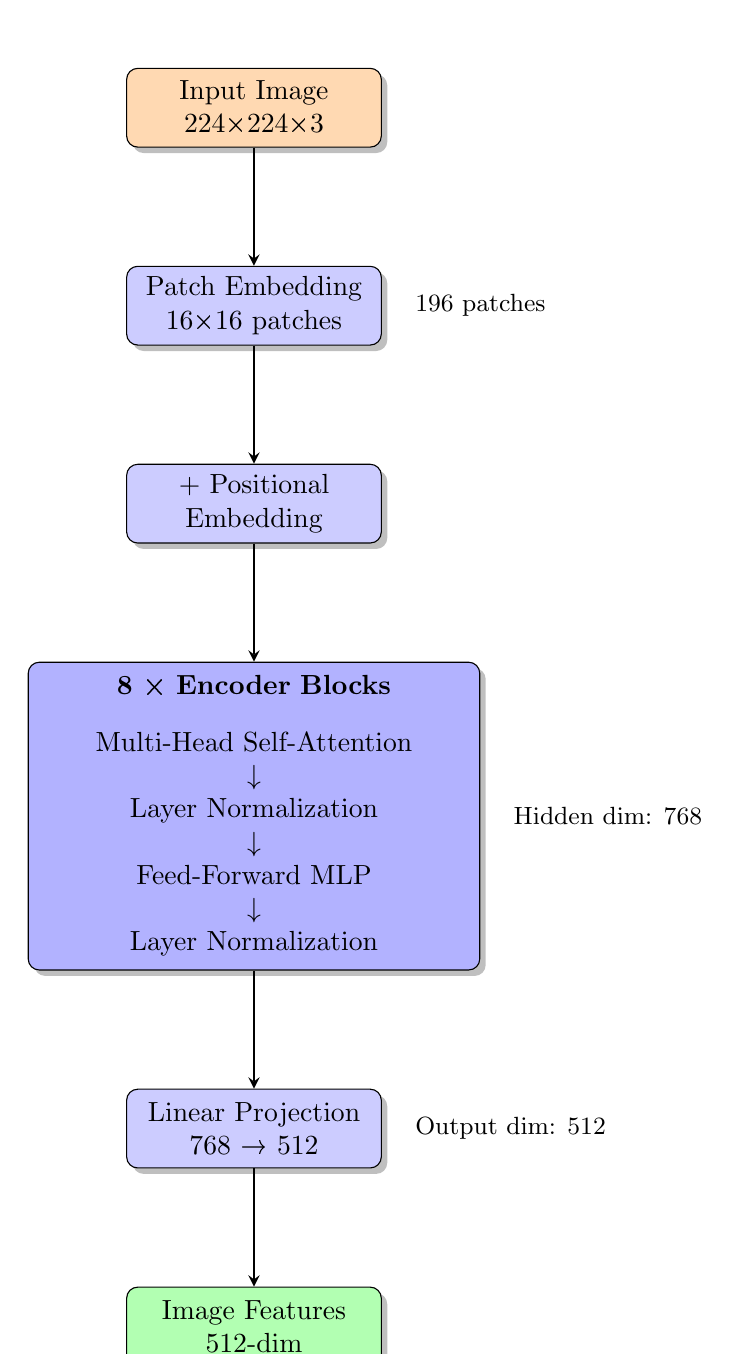
\begin{tikzpicture}[
    node distance=1.5cm and 2cm,
    block/.style={rectangle, draw, fill=blue!20, text width=3cm, text centered, rounded corners, minimum height=1cm, drop shadow},
    smallblock/.style={rectangle, draw, fill=green!20, text width=2.5cm, text centered, rounded corners, minimum height=0.8cm, drop shadow},
    arrow/.style={->, >=stealth, thick},
    label/.style={font=\small}
]

% Input
\node[block, fill=orange!30] (input) {Input Image\\224×224×3};

% Patch Embedding
\node[block, below=of input] (patch) {Patch Embedding\\16×16 patches};
\node[label, right=0.3cm of patch] {196 patches};

% Positional Encoding
\node[block, below=of patch] (pos) {+ Positional\\Embedding};

% Encoder Blocks Container
\node[block, below=of pos, minimum height=2.5cm, fill=blue!30, text width=5.5cm] (encoder) {
    \begin{tabular}{c}
    \textbf{8 × Encoder Blocks}\\[0.3cm]
    Multi-Head Self-Attention\\
    $\downarrow$\\
    Layer Normalization\\
    $\downarrow$\\
    Feed-Forward MLP\\
    $\downarrow$\\
    Layer Normalization
    \end{tabular}
};

% Dimension Reduction
\node[block, below=of encoder] (proj) {Linear Projection\\768 → 512};

% Output
\node[block, below=of proj, fill=green!30] (output) {Image Features\\512-dim};

% Arrows
\draw[arrow] (input) -- (patch);
\draw[arrow] (patch) -- (pos);
\draw[arrow] (pos) -- (encoder);
\draw[arrow] (encoder) -- (proj);
\draw[arrow] (proj) -- (output);

% Side annotations
\node[label, right=0.3cm of encoder] {Hidden dim: 768};
\node[label, right=0.3cm of proj] {Output dim: 512};

\end{tikzpicture}
\caption{Vision Transformer Encoder Architecture}
\label{fig:vit-encoder}
\end{figure}

\textbf{Key Components:}

\begin{enumerate}
\item \textbf{Patch Embedding:} The input image (224×224×3) is divided into 196 non-overlapping 16×16 patches. Each patch is projected to a $16^2 \times 3 = 768$-dimensional embedding vector via a convolutional layer.

\item \textbf{Class Token + Positional Embedding:} A learnable [CLS] token is prepended to the 196 patch embeddings, and learnable positional embeddings are added to all 197 tokens to preserve spatial information.

\item \textbf{Multi-Head Self-Attention (MSA):} Each encoder block contains multi-head self-attention with \textbf{4 attention heads}. This allows the model to attend to different regions of the image simultaneously, capturing both local details and global context.

\item \textbf{Feed-Forward Network:} After attention, features pass through a two-layer MLP with GELU activation, expanding to $768 \times 4 = 3072$ dimensions internally before projecting back to 768.

\item \textbf{Layer Normalization:} Applied after each sub-layer (post-norm architecture) for training stability.

\item \textbf{Residual Connections:} Skip connections around each sub-layer help gradient flow during backpropagation.

\item \textbf{Output:} The [CLS] token representation (768-dim) is extracted and projected to 512-dim via a linear layer before being passed to the GPT-2 decoder.
\end{enumerate}

\subsubsection{GPT-2 Decoder}
The decoder generates captions autoregressively using the image features:

\begin{figure}[H]
\centering
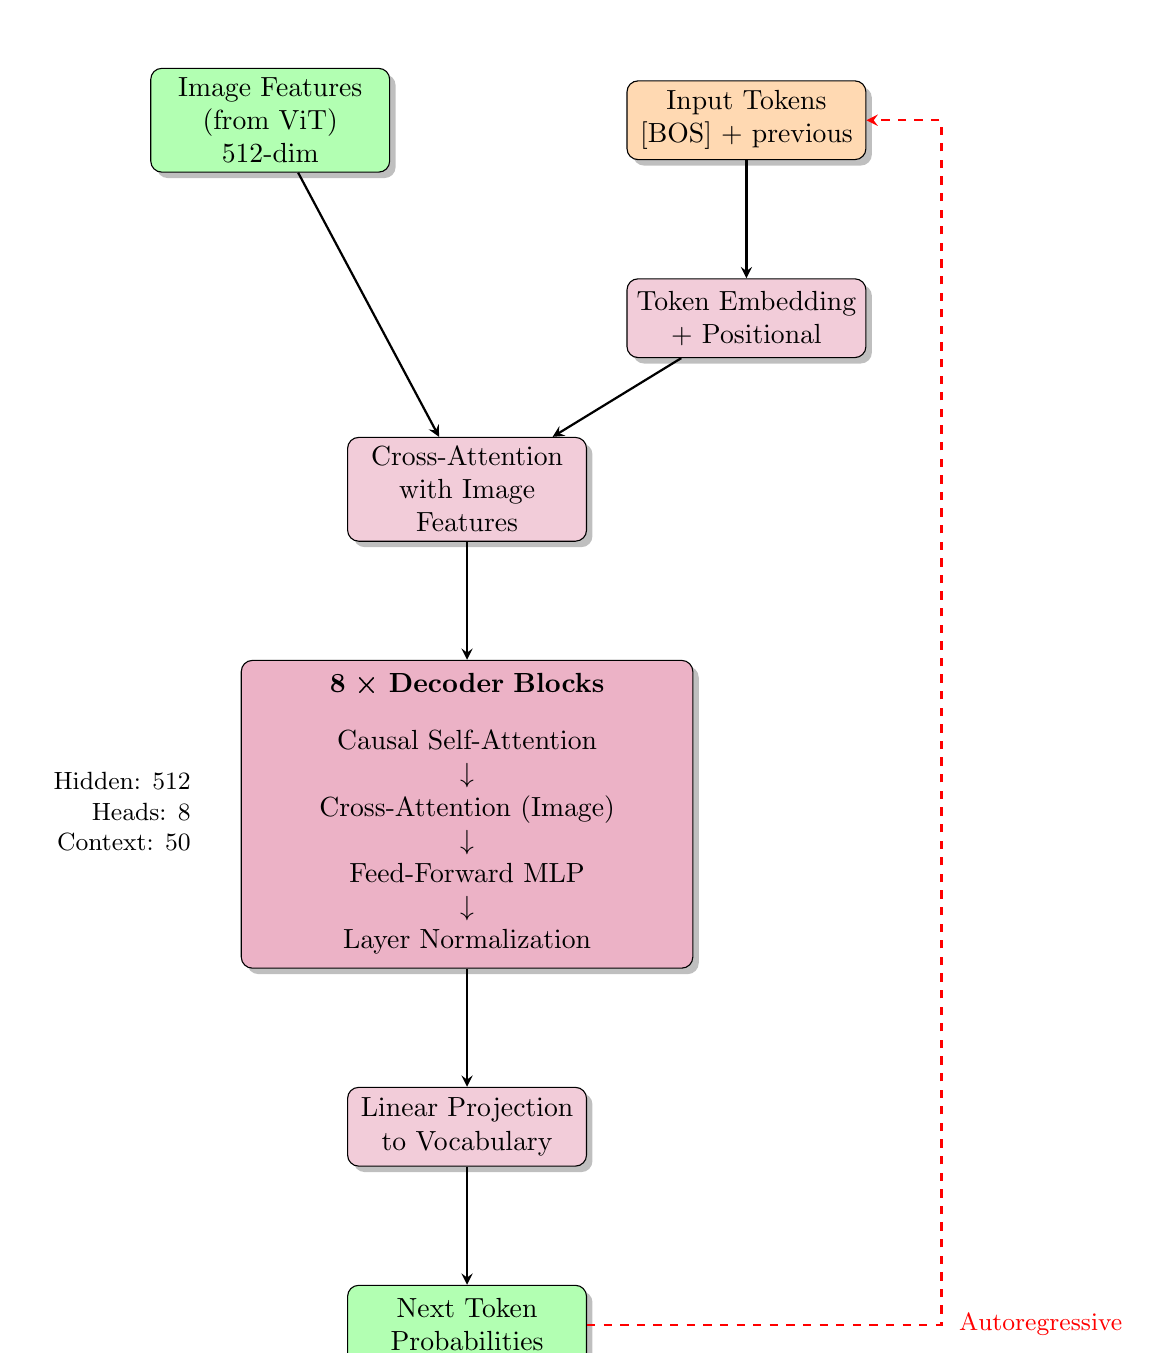
\begin{tikzpicture}[
    node distance=1.5cm and 1.5cm,
    block/.style={rectangle, draw, fill=purple!20, text width=2.8cm, text centered, rounded corners, minimum height=1cm, drop shadow},
    arrow/.style={->, >=stealth, thick},
    label/.style={font=\small}
]

% Image features input
\node[block, fill=green!30] (imgfeat) {Image Features\\(from ViT)\\512-dim};

% Token input
\node[block, right=3cm of imgfeat, fill=orange!30] (tokens) {Input Tokens\\{[BOS]} + previous};

% Token Embedding
\node[block, below=of tokens] (embed) {Token Embedding\\+ Positional};

% Cross Attention with Image
\node[block, below left=1cm and 0.5cm of embed] (cross) {Cross-Attention\\with Image Features};

% Decoder blocks
\node[block, below=of cross, minimum height=3cm, fill=purple!30, text width=5.5cm] (decoder) {
    \begin{tabular}{c}
    \textbf{8 × Decoder Blocks}\\[0.3cm]
    Causal Self-Attention\\
    $\downarrow$\\
    Cross-Attention (Image)\\
    $\downarrow$\\
    Feed-Forward MLP\\
    $\downarrow$\\
    Layer Normalization
    \end{tabular}
};

% Output projection
\node[block, below=of decoder] (proj) {Linear Projection\\to Vocabulary};

% Output
\node[block, below=of proj, fill=green!30] (output) {Next Token\\Probabilities};

% Arrows
\draw[arrow] (imgfeat) -- (cross);
\draw[arrow] (tokens) -- (embed);
\draw[arrow] (embed) -- (cross);
\draw[arrow] (cross) -- (decoder);
\draw[arrow] (decoder) -- (proj);
\draw[arrow] (proj) -- (output);

% Autoregressive loop
\draw[arrow, dashed, red] (output.east) -- ++(4.5,0) |- (tokens.east);
\node[label, red, right=4.6cm of output] {Autoregressive};

% Side annotations
\node[label, left=0.3cm of decoder] {\begin{tabular}{r}Hidden: 512\\Heads: 8\\Context: 50\end{tabular}};

\end{tikzpicture}
\caption{GPT-2 Decoder Architecture for Caption Generation}
\label{fig:gpt-decoder}
\end{figure}

\textbf{Key Components:}

\begin{enumerate}
\item \textbf{Token Embedding:} Input tokens are embedded into 512-dimensional vectors via a learned embedding table (GPT-2 tokenizer vocabulary of 50,257 + 3 special tokens = 50,260 tokens), combined with learned positional embeddings (context length 50).

\item \textbf{Causal Self-Attention:} Custom masked self-attention with \textbf{8 attention heads} and safe softmax ensures that each position can only attend to previous positions, maintaining the autoregressive property. A custom causal mask combined with padding mask is applied.

\item \textbf{Cross-Attention with Image:} Each decoder block attends to the projected image features (512-dim, from ViT's [CLS] token), allowing the model to ground generated text in visual content.

\item \textbf{Autoregressive Generation:} Starting with [BOS] token, the model generates one token at a time, feeding each generated token back as input (greedy decoding via argmax) until [EOS] token is produced or maximum length (50 tokens) is reached.
\end{enumerate}

\subsection{Complete Emotion-Aware Pipeline}

The following diagram shows the end-to-end pipeline integrating all three components:

\begin{figure}[H]
\centering
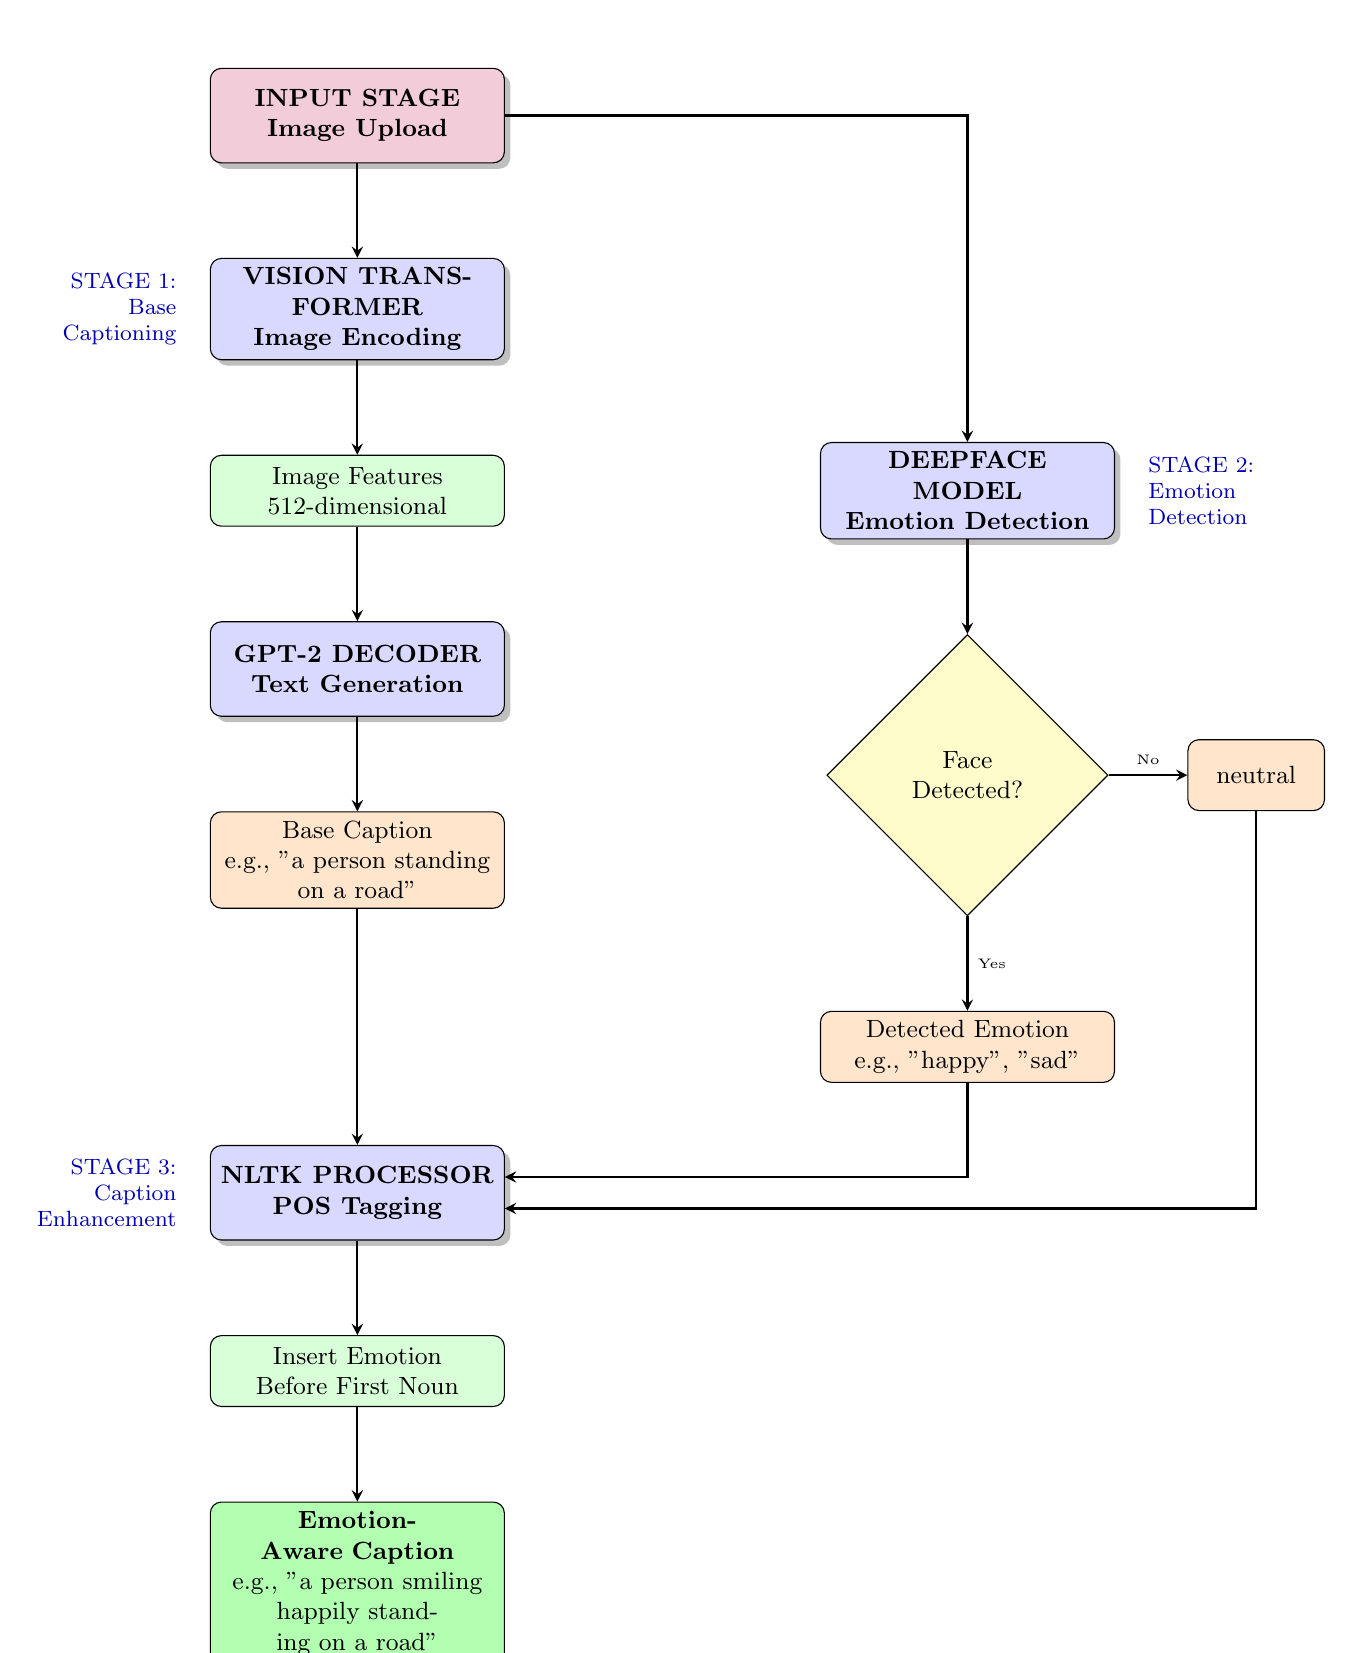
\begin{tikzpicture}[
    node distance=1.2cm and 1.5cm,
    stage/.style={rectangle, draw, fill=blue!15, text width=3.5cm, text centered, rounded corners, minimum height=1.2cm, drop shadow, font=\small\bfseries},
    process/.style={rectangle, draw, fill=green!15, text width=3.5cm, text centered, rounded corners, minimum height=0.9cm, font=\small},
    output/.style={rectangle, draw, fill=orange!20, text width=3.5cm, text centered, rounded corners, minimum height=0.9cm, font=\small},
    decision/.style={diamond, draw, fill=yellow!20, text width=2.5cm, text centered, minimum height=1cm, font=\small},
    arrow/.style={->, >=stealth, thick},
    label/.style={font=\footnotesize, text=blue!70!black}
]

% Stage 1: Input
\node[stage, fill=purple!20] (input) {INPUT STAGE\\Image Upload};

% Stage 2: Base Captioning
\node[stage, below=of input] (vit) {VISION TRANSFORMER\\Image Encoding};
\node[process, below=of vit] (vitout) {Image Features\\512-dimensional};
\node[stage, below=of vitout] (gpt) {GPT-2 DECODER\\Text Generation};
\node[output, below=of gpt] (basecap) {Base Caption\\e.g., "a person standing\\on a road"};

% Stage 3: Emotion Detection
\node[stage, right=4cm of vitout] (deepface) {DEEPFACE MODEL\\Emotion Detection};
\node[decision, below=of deepface] (detect) {Face\\Detected?};
\node[output, below=of detect] (emotion) {Detected Emotion\\e.g., "happy", "sad"};
\node[output, right=1cm of detect, text width=1.5cm] (noemot) {neutral};

% Stage 4: Emotion Integration  
\node[stage, below=3cm of basecap] (nltk) {NLTK PROCESSOR\\POS Tagging};
\node[process, below=of nltk] (insert) {Insert Emotion\\Before First Noun};
\node[output, below=of insert, fill=green!30] (final) {\textbf{Emotion-Aware Caption}\\e.g., "a person smiling\\happily standing on a road"};

% Arrows - Main flow
\draw[arrow] (input) -- (vit);
\draw[arrow] (vit) -- (vitout);
\draw[arrow] (vitout) -- (gpt);
\draw[arrow] (gpt) -- (basecap);

% Arrows - Emotion detection
\draw[arrow] (input.east) -| (deepface.north);
\draw[arrow] (deepface) -- (detect);
\draw[arrow] (detect) -- node[right, font=\tiny] {Yes} (emotion);
\draw[arrow] (detect) -- node[above, font=\tiny] {No} (noemot);

% Arrows - Integration
\draw[arrow] (basecap) -- (nltk);
\draw[arrow] (emotion.south) |- ([yshift=0.2cm]nltk.east);
\draw[arrow] (noemot.south) |- ([yshift=-0.2cm]nltk.east);
\draw[arrow] (nltk) -- (insert);
\draw[arrow] (insert) -- (final);

% Stage labels
\node[label, left=0.3cm of vit, align=right] {STAGE 1:\\Base\\Captioning};
\node[label, right=0.3cm of deepface, align=left] {STAGE 2:\\Emotion\\Detection};
\node[label, left=0.3cm of nltk, align=right] {STAGE 3:\\Caption\\Enhancement};

\end{tikzpicture}
\caption{Complete Emotion-Aware Image Captioning Pipeline}
\label{fig:complete-pipeline}
\end{figure}

\subsection{Emotion Detection: DeepFace}

We employ the DeepFace framework for facial emotion recognition. DeepFace is a state-of-the-art deep learning model pre-trained on large-scale facial datasets.

\textbf{Emotion Categories:}
\begin{itemize}
\item Happy
\item Sad  
\item Angry
\item Surprise
\item Fear
\item Disgust
\item Neutral
\end{itemize}

\textbf{Processing Steps:}
\begin{enumerate}
\item Image is temporarily saved as JPEG file
\item DeepFace analyzes the image with \texttt{enforce\_detection=False} to handle edge cases
\item Dominant emotion is extracted from the analysis result
\item If detection fails, defaults to "neutral"
\end{enumerate}

\subsection{Emotion Integration: NLTK-based Grammatical Insertion}

To ensure natural-sounding captions, we developed a grammatical insertion mechanism using NLTK's part-of-speech tagging:

\textbf{Emotion-to-Adjective Mapping:}
\begin{center}
\begin{tabular}{ll}
\toprule
\textbf{Emotion} & \textbf{Adjective (Inserted)} \\
\midrule
Happy & joyful \\
Sad & melancholic \\
Angry & angry \\
Surprise & surprised \\
Fear & fearful \\
Disgust & disgusted \\
Neutral & calm \\
\bottomrule
\end{tabular}
\end{center}

\textbf{Insertion Algorithm:}
\begin{enumerate}
\item Tokenize the base caption into words
\item Apply POS tagging to identify grammatical roles
\item Locate the first noun (tag starting with 'NN')
\item Insert emotion adjective immediately before the first noun
\item Reconstruct the caption with proper spacing
\end{enumerate}

\textbf{Example:}
\begin{itemize}
\item \textbf{Input:} "a person standing on a road", emotion: "happy"
\item \textbf{POS Tags:} [('a', 'DT'), ('person', 'NN'), ('standing', 'VBG'), ('on', 'IN'), ('a', 'DT'), ('road', 'NN')]
\item \textbf{First noun:} 'person' at position 1
\item \textbf{Insertion:} Insert 'joyful' at position 1
\item \textbf{Output:} "a joyful person standing on a road"
\end{itemize}

%%%%%%%%%%%%%%%%%%%%%%%%%%%%%%%%%%%%%%%%%%%%%%%%%%%%%%%%%%%%%%%%%%%%%
\section{Dataset and Training}
%%%%%%%%%%%%%%%%%%%%%%%%%%%%%%%%%%%%%%%%%%%%%%%%%%%%%%%%%%%%%%%%%%%%%

\subsection{Flickr30k Dataset}
We used the Flickr30k dataset, a widely-adopted benchmark for image captioning research.

\textbf{Dataset Statistics:}
\begin{itemize}
\item \textbf{Total Images:} 8,091 images
\item \textbf{Total Captions:} Approximately 40,455 (5 captions per image; one caption per image used after de-duplication)
\item \textbf{Content:} Diverse real-world scenes with people, animals, objects, and activities
\item \textbf{Source:} Kaggle (flickr-image-dataset, publicly available)
\end{itemize}

\textbf{Data Split (as implemented in code):}
\begin{center}
\begin{tabular}{lrr}
\toprule
\textbf{Split} & \textbf{Images (approx.)} & \textbf{Percentage} \\
\midrule
Training & $\sim$6,473 & 80\% \\
Test & $\sim$1,618 & 20\% \\
\bottomrule
\end{tabular}
\end{center}
\textit{Note: No separate validation split is used; the 80/20 train-test split is applied randomly at runtime.}

\subsection{Training Configuration}

\begin{metricbox}
\textbf{Training Hyperparameters:}
\begin{itemize}
\item \textbf{Total Epochs:} 20
\item \textbf{Frozen Epochs:} 2 (ViT encoder frozen, only GPT-2 decoder + projection layer trained)
\item \textbf{Fine-tuning Epochs:} 18 (end-to-end training with full model)
\item \textbf{Batch Size:} 16
\item \textbf{Learning Rate:} 2e-4
\item \textbf{Optimizer:} Adam (with weight decay $10^{-6}$)
\item \textbf{Dropout:} 0.5 (applied to attention, MLP, and embeddings)
\item \textbf{Context Length:} 50 tokens
\item \textbf{Vocabulary Size:} GPT-2 tokenizer (50,257 tokens) + 3 special tokens ([BOS], [EOS], [PAD]) = 50,260
\end{itemize}
\end{metricbox}

\textbf{Training Strategy:}
\begin{enumerate}
\item \textbf{Phase 1 (Epochs 1--2):} ViT encoder weights are frozen. Only the GPT-2 decoder and the 768→512 linear projection layer are trained. The ViT learning rate is set to 0 while the decoder learning rate is $2\times10^{-4}$. This stabilizes early training.

\item \textbf{Phase 2 (Epochs 3--20):} All weights are unfrozen and the full model is trained end-to-end with the same learning rate of $2\times10^{-4}$. Both encoder and decoder adapt jointly to the captioning task.
\end{enumerate}

\textbf{Computational Resources:}
\begin{itemize}
\item \textbf{Platform:} Kaggle GPU (NVIDIA Tesla T4)
\item \textbf{Training Time:} Approximately 6--8 hours total (20 epochs)
\item \textbf{Model Size:} $\sim$500MB (.pt checkpoint file)
\item \textbf{Parameters:} $\sim$131 million (ViT-Base encoder + custom GPT-2 decoder + projection layer)
\end{itemize}

%%%%%%%%%%%%%%%%%%%%%%%%%%%%%%%%%%%%%%%%%%%%%%%%%%%%%%%%%%%%%%%%%%%%%
\section{Implementation Details}
%%%%%%%%%%%%%%%%%%%%%%%%%%%%%%%%%%%%%%%%%%%%%%%%%%%%%%%%%%%%%%%%%%%%%

\subsection{Model Architecture Implementation}

Our implementation consists of several key modules:

\subsubsection{Vision Transformer (vit.py)}
\begin{itemize}
\item \texttt{PatchEmbeddings}: Converts image to patch sequences
\item \texttt{ViTEmbedding}: Combines patch and positional embeddings
\item \texttt{MSABlock}: Multi-head self-attention with 8 heads
\item \texttt{EncoderBlock}: Complete transformer encoder layer
\item \texttt{ViT}: Full Vision Transformer with 8 encoder blocks
\end{itemize}

\subsubsection{GPT-2 Decoder (gpt.py)}
\begin{itemize}
\item \texttt{GPTEmbedding}: Token and positional embeddings
\item \texttt{CausalSelfAttnBlock}: Masked self-attention for autoregressive generation
\item \texttt{CrossAttnBlock}: Attention over image features
\item \texttt{GPTDecoderBlock}: Combined causal + cross attention layer
\item \texttt{GPT}: Complete decoder with 8 blocks
\end{itemize}

\subsubsection{Caption Model (caption\_model.py)}
\begin{itemize}
\item \texttt{ImageCaptionModel}: Combines ViT encoder and GPT decoder
\item \texttt{generate()}: Autoregressive beam search for caption generation
\item Support for custom special tokens ([BOS], [EOS], [PAD])
\end{itemize}

\subsubsection{Emotion Processing (emotion.py)}
\begin{itemize}
\item \texttt{detect\_emotion\_deepface()}: Facial emotion detection using DeepFace
\item \texttt{insert\_emotion\_in\_caption()}: NLTK-based grammatical insertion
\item \texttt{generate\_emotion\_aware\_caption()}: End-to-end pipeline
\end{itemize}

\subsection{Dependencies}
\begin{itemize}
\item \textbf{Deep Learning:} PyTorch 2.0.1, torchvision 0.15.2
\item \textbf{Transformers:} transformers 4.28.0, timm 0.9.2
\item \textbf{NLP:} NLTK 3.8.1 (punkt, averaged\_perceptron\_tagger)
\item \textbf{Emotion Detection:} deepface 0.0.79, tensorflow 2.13.0
\item \textbf{Image Processing:} Pillow 10.0.0, opencv-python-headless 4.8.0
\item \textbf{Web Framework:} FastAPI 0.95.0, uvicorn 0.21.0
\end{itemize}

%%%%%%%%%%%%%%%%%%%%%%%%%%%%%%%%%%%%%%%%%%%%%%%%%%%%%%%%%%%%%%%%%%%%%
\section{Evaluation Metrics and Results}
%%%%%%%%%%%%%%%%%%%%%%%%%%%%%%%%%%%%%%%%%%%%%%%%%%%%%%%%%%%%%%%%%%%%%

\subsection{Evaluation Methodology}

We evaluate our base captioning system using standard metrics:

\begin{metricbox}
\textbf{BLEU (Bilingual Evaluation Understudy):}
Measures n-gram overlap between generated and reference captions. BLEU-1 through BLEU-4 evaluate unigram to 4-gram precision.

\textbf{METEOR (Metric for Evaluation of Translation with Explicit ORdering):}
Considers synonyms and stems, providing more nuanced evaluation than BLEU. Balances precision and recall with emphasis on recall.

\textbf{Evaluation Set:}
Tested on Flickr30k test split (1,091 images, 5,455 reference captions)
\end{metricbox}

\subsection{Quantitative Results}

\begin{resultbox}
\textbf{Our Model Performance:}
\begin{center}
\begin{tabular}{lcc}
\toprule
\textbf{Metric} & \textbf{Our Score} & \textbf{Paper Baseline} \\
\midrule
BLEU-1 & \textbf{0.5947} & 0.5834 \\
BLEU-2 & \textbf{0.4060} & 0.4023 \\
BLEU-3 & 0.2879 & \textbf{0.2911} \\
BLEU-4 & 0.2096 & \textbf{0.2154} \\
METEOR & \textbf{0.2538} & 0.2483 \\
\bottomrule
\end{tabular}
\end{center}
\end{resultbox}

\textbf{Analysis:}
\begin{itemize}
\item Our model achieves \textbf{competitive performance} with the reference paper~\cite{sankhla2024}
\item \textbf{Superior BLEU-1 and BLEU-2:} Better performance on unigram and bigram precision indicates stronger word-level accuracy
\item \textbf{Higher METEOR score:} Suggests better semantic alignment and synonym handling
\item Slightly lower BLEU-3 and BLEU-4 indicate room for improvement in longer phrase generation
\item Overall results validate our implementation's effectiveness for base caption generation
\end{itemize}

\subsection{Qualitative Results: Emotion-Aware Captions}

This section presents qualitative examples of emotion-aware captions generated by our system.
We tested the complete pipeline on a variety of images containing human faces,
and we showed some of the examples here.

\begin{figure}[H]
\centering
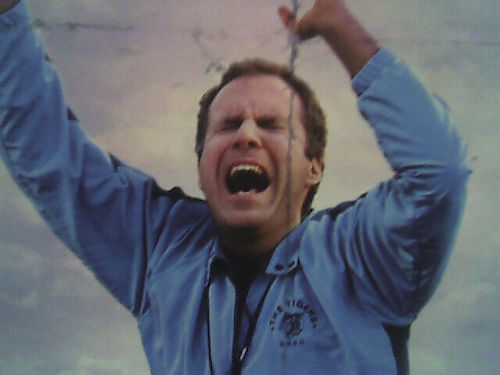
\includegraphics[width=0.9\textwidth]{images/15085612.jpg}
\caption*{\textbf{Base Caption:} A young man with dark hair and a blue shirt is raising his hand up in the air .\\
\textbf{Detected Emotion:} sad\\
\textbf{Emotion-Aware Caption:} A young melancholic man with dark hair and a blue shirt is raising his hand up in the air .}
\end{figure}

\begin{figure}[H]
\centering
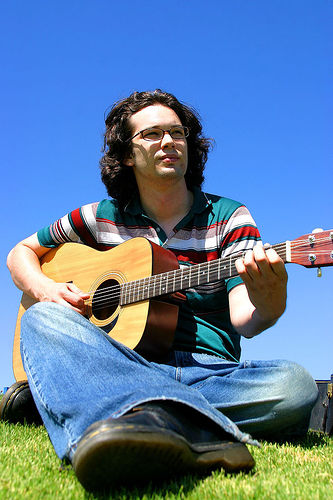
\includegraphics[width=0.9\textwidth]{images/23770160.jpg}
\caption*{\textbf{Base Caption:} A man with long hair and a long-sleeved shirt plays guitar on a sunny day .\\
\textbf{Detected Emotion:} neutral\\
\textbf{Emotion-Aware Caption:} A calm man with long hair and a long-sleeved shirt plays guitar on a sunny day .}
\end{figure}

\begin{figure}[H]
\centering
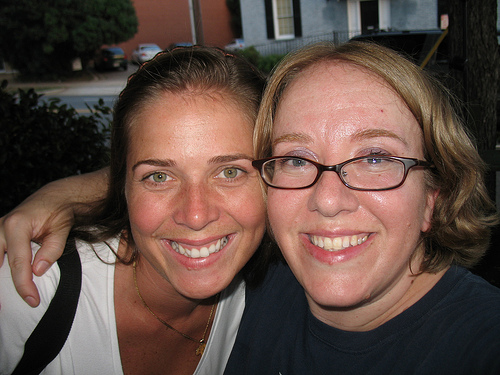
\includegraphics[width=0.9\textwidth]{images/Happy_2.jpg}
\caption*{\textbf{Base Caption:} Two women with their arms around each other\\
\textbf{Detected Emotion:} happy\\
\textbf{Emotion-Aware Caption:} Two joyful women with their arms around each other}
\end{figure}

\begin{figure}[H]
\centering
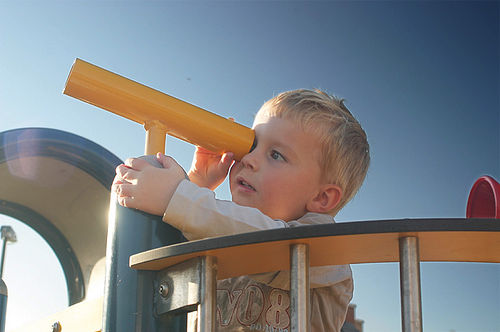
\includegraphics[width=0.9\textwidth]{images/6155176.jpg}
\caption*{\textbf{Base Caption:} A little boy in a yellow shirt is looking through the telescope at the playground .\\
\textbf{Detected Emotion:} neutral\\
\textbf{Emotion-Aware Caption:} A little calm boy in a yellow shirt is looking through the telescope at the playground .}
\end{figure}

\begin{figure}[H]
\centering
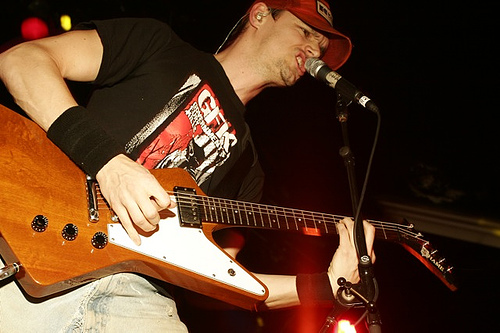
\includegraphics[width=0.9\textwidth]{images/Angry_1.jpg}
\caption*{\textbf{Base Caption:} A man in a red shirt is playing guitar and singing into a microphone .\\
\textbf{Detected Emotion:} angry\\
\textbf{Emotion-Aware Caption:} A angry man in a red shirt is playing guitar and singing into a microphone .}
\end{figure}

\begin{figure}[H]
\centering
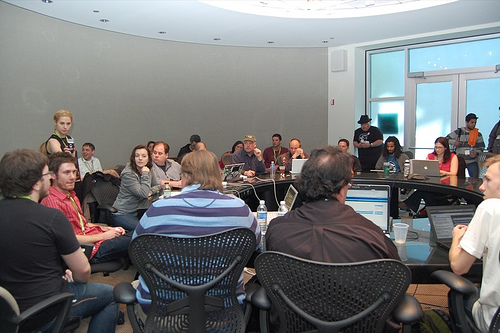
\includegraphics[width=0.9\textwidth]{images/Neutral_8.jpg}
\caption*{\textbf{Base Caption:} A group of people are sitting at a table with a computer screen in the background .\\
\textbf{Detected Emotion:} neutral\\
\textbf{Emotion-Aware Caption:} A calm group of people are sitting at a table with a computer screen in the background .}
\end{figure}

\begin{figure}[H]
\centering
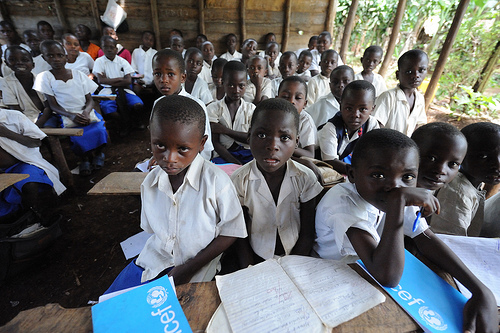
\includegraphics[width=0.9\textwidth]{images/Disgust_1.jpg}
\caption*{\textbf{Base Caption:} A group of students are watching a conference performance in a fancy class .\\
\textbf{Detected Emotion:} disgust\\
\textbf{Emotion-Aware Caption:} A disgusted group of students are watching a conference performance in a fancy class .}
\end{figure}

\begin{figure}[H]
\centering
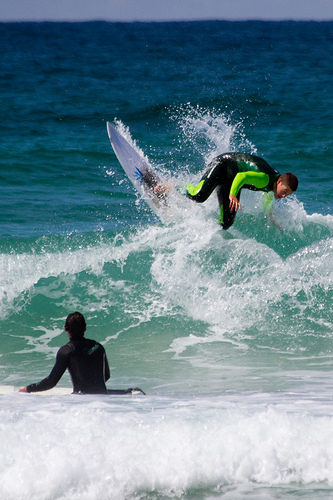
\includegraphics[width=0.9\textwidth]{images/Fear_7.jpg}
\caption*{\textbf{Base Caption:} A surfer in a black wetsuit surfs in the ocean with a wave in the background .\\
\textbf{Detected Emotion:} fear\\
\textbf{Emotion-Aware Caption:} A fearful surfer in a black wetsuit surfs in the ocean with a wave in the background .}
\end{figure}

\begin{figure}[H]
\centering
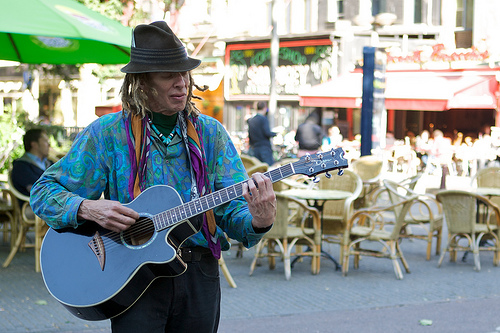
\includegraphics[width=0.9\textwidth]{images/Happy_4.jpg}
\caption*{\textbf{Base Caption:} A man in a colorful outfit with a long hair and wearing a black and blue plaid shirt is playing a guitar .\\
\textbf{Detected Emotion:} happy\\
\textbf{Emotion-Aware Caption:} A joyful man in a colorful outfit with a long hair and wearing a black and blue plaid shirt is playing a guitar .}
\end{figure}

\begin{figure}[H]
\centering
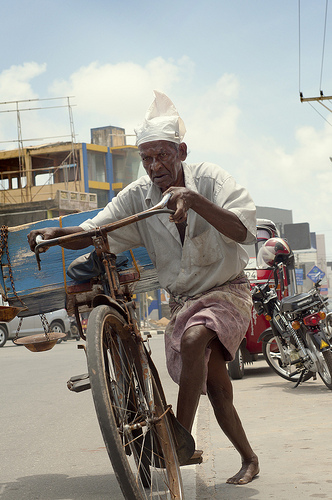
\includegraphics[width=0.9\textwidth]{images/8118985445.jpg}
\caption*{\textbf{Base Caption:} A man riding a bicycle down the street in a warm neighborhood , with a basket of bicycles in the background .\\
\textbf{Detected Emotion:} sad\\
\textbf{Emotion-Aware Caption:} A melancholic man riding a bicycle down the street in a warm neighborhood , with a basket of bicycles in the background .}
\end{figure}

\begin{figure}[H]
\centering
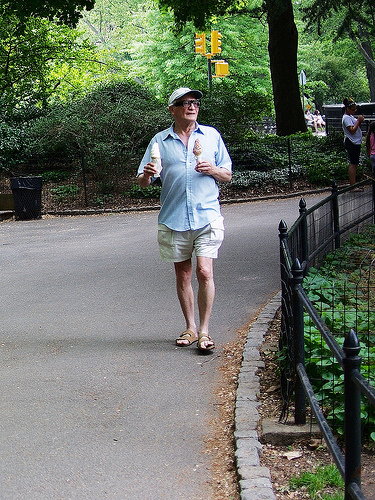
\includegraphics[width=0.9\textwidth]{images/4756254503.jpg}
\caption*{\textbf{Base Caption:} A man wearing shorts and a white t-shirt walks down the sidewalk with a cane in his hand .\\
\textbf{Detected Emotion:} happy\\
\textbf{Emotion-Aware Caption:} A joyful man wearing shorts and a white t-shirt walks down the sidewalk with a cane in his hand .}
\end{figure}

\begin{figure}[H]
\centering
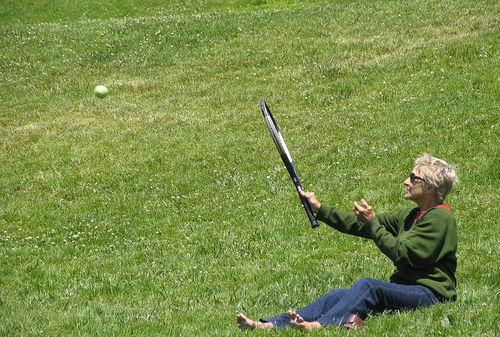
\includegraphics[width=0.9\textwidth]{images/18119750.jpg}
\caption*{\textbf{Base Caption:} A woman in a green sweatshirt and jeans is sitting on a lawn with a tennis ball in her hand .\\
\textbf{Detected Emotion:} neutral\\
\textbf{Emotion-Aware Caption:} A calm woman in a green sweatshirt and jeans is sitting on a lawn with a tennis ball in her hand .}
\end{figure}

\begin{figure}[H]
\centering
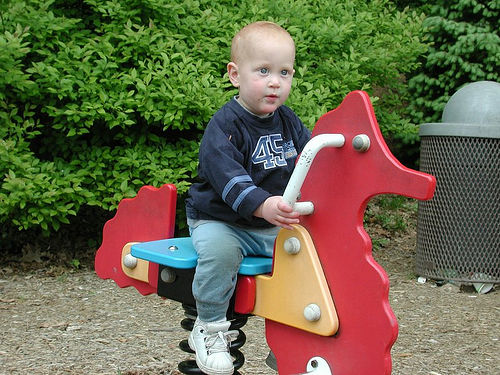
\includegraphics[width=0.9\textwidth]{images/15859665.jpg}
\caption*{\textbf{Base Caption:} A small child is riding on a bouncy toy that is in the park .\\
\textbf{Detected Emotion:} fear\\
\textbf{Emotion-Aware Caption:} A small fearful child is riding on a bouncy toy that is in the park .}
\end{figure}

\begin{figure}[H]
\centering
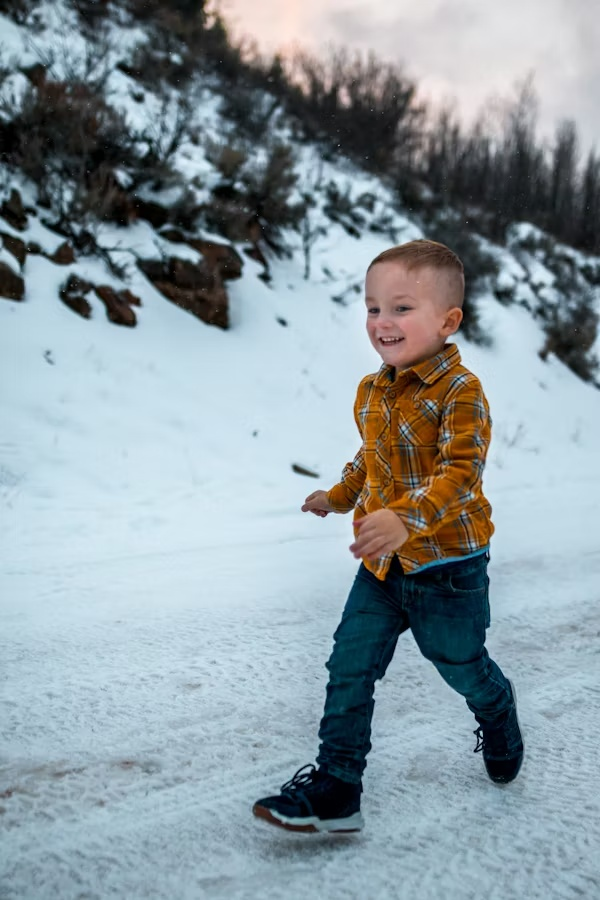
\includegraphics[width=0.9\textwidth]{images/happy_3.jpg}
\caption*{\textbf{Base Caption:} A young boy in a yellow jacket and blue jeans walks in the snow .\\
\textbf{Detected Emotion:} happy\\
\textbf{Emotion-Aware Caption:} A young joyful boy in a yellow jacket and blue jeans walks in the snow .}
\end{figure}

\begin{figure}[H]
\centering
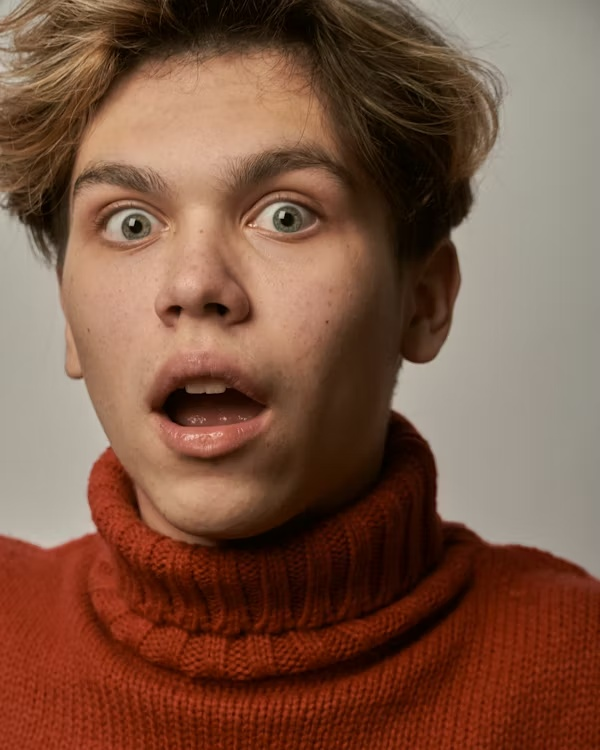
\includegraphics[width=0.9\textwidth]{images/surprise_1.jpg}
\caption*{\textbf{Base Caption:} A young boy with brown eyes and a white shirt is looking at the camera .\\
\textbf{Detected Emotion:} surprise\\
\textbf{Emotion-Aware Caption:} A young surprised boy with brown eyes and a white shirt is looking at the camera .}
\end{figure}

\begin{figure}[H]
\centering

\includegraphics[width=0.9\textwidth]{images/fear_cus_2.jpg}
\caption*{\textbf{Base Caption:} A black man with glasses and a black shirt is standing in front of a white wall .\\
\textbf{Detected Emotion:} fear\\
\textbf{Emotion-Aware Caption:} A black fearful man with glasses and a black shirt is standing in front of a white wall .}
\end{figure}

\begin{figure}[H]
\centering
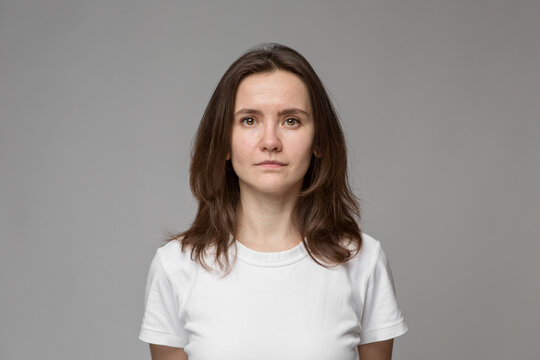
\includegraphics[width=0.9\textwidth]{images/nuetral_bus_1.jpg}
\caption*{\textbf{Base Caption:} A young girl in a white dress and a necklace is standing in front of a white wall .\\
\textbf{Detected Emotion:} neutral\\
\textbf{Emotion-Aware Caption:} A young calm girl in a white dress and a necklace is standing in front of a white wall .}
\end{figure}

\begin{figure}[H]
\centering
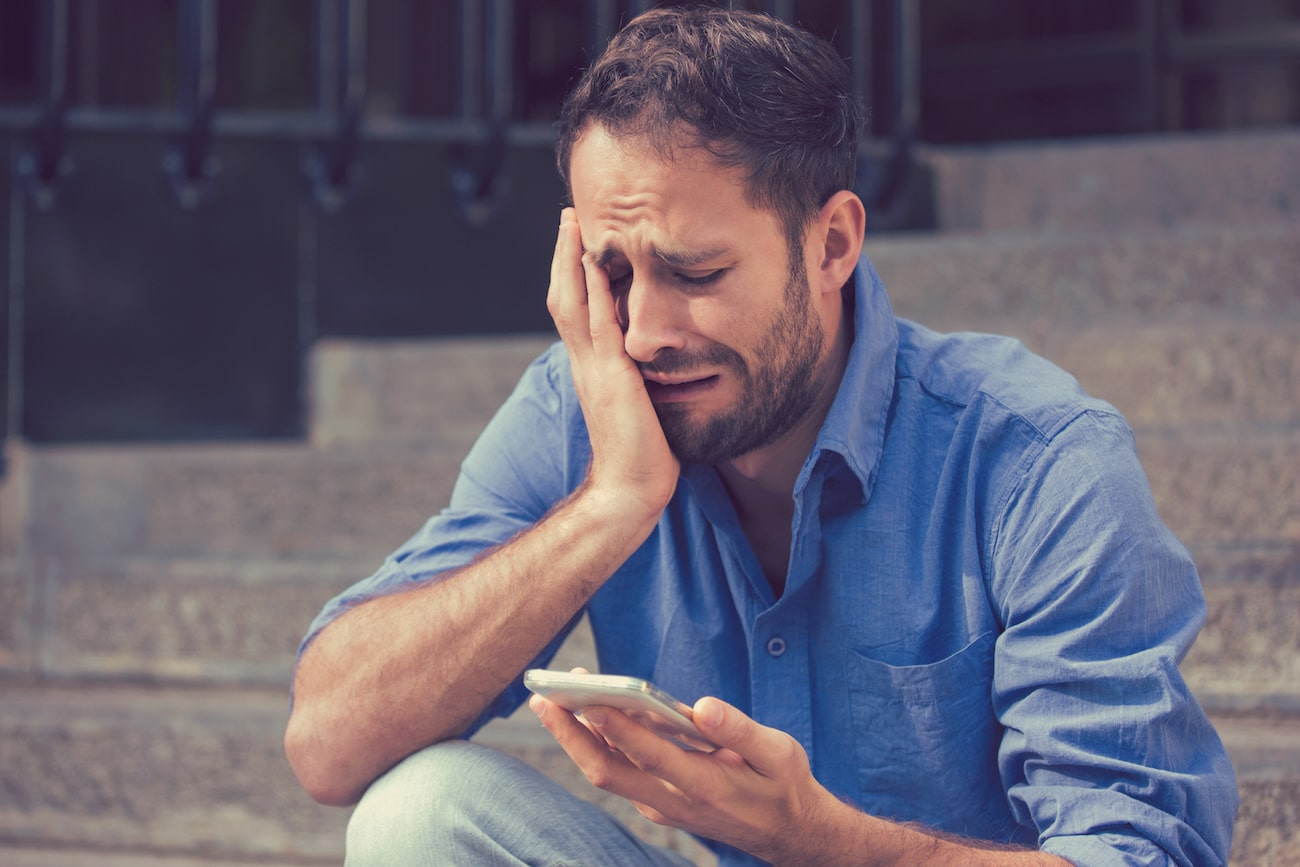
\includegraphics[width=0.9\textwidth]{images/sad_cus_1.jpeg}
\caption*{\textbf{Base Caption:} A man in a blue shirt and glasses sits on the ground with his eyes closed .\\
\textbf{Detected Emotion:} fear\\
\textbf{Emotion-Aware Caption:} A fearful man in a blue shirt and glasses sits on the ground with his eyes closed .}
\end{figure}

\begin{figure}[H]
\centering

\includegraphics[width=0.9\textwidth]{images/surprise_cus_2.jpg}
\caption*{\textbf{Base Caption:} A blond-haired toddler is sitting in a highchair .\\
\textbf{Detected Emotion:} surprise\\
\textbf{Emotion-Aware Caption:} A blond-haired surprised toddler is sitting in a highchair .}
\end{figure}

\begin{figure}[H]
\centering
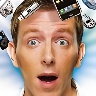
\includegraphics[width=0.9\textwidth]{images/Aff_Surprise_1.jpg}
\caption*{\textbf{Base Caption:} A young boy with dark hair and a large smile at the camera .\\
\textbf{Detected Emotion:} surprise\\
\textbf{Emotion-Aware Caption:} A young surprised boy with dark hair and a large smile at the camera .}
\end{figure}

\begin{figure}[H]
\centering
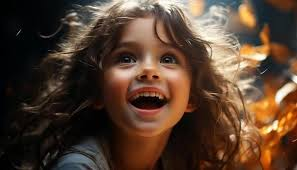
\includegraphics[width=0.9\textwidth]{images/5.jpg}
\caption*{\textbf{Base Caption:} A girl with long brown hair and a bright smile at the camera .\\
\textbf{Detected Emotion:} happy\\
\textbf{Emotion-Aware Caption:} A joyful girl with long brown hair and a bright smile at the camera .}
\end{figure}

\begin{figure}[H]
\centering
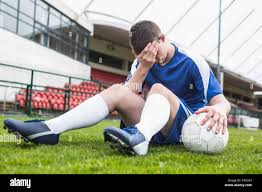
\includegraphics[width=0.9\textwidth]{images/20.jpg}
\caption*{\textbf{Base Caption:} A man in a blue shirt and shorts is sitting on a grassy hill .\\
\textbf{Detected Emotion:} sad\\
\textbf{Emotion-Aware Caption:} A melancholic man in a blue shirt and shorts is sitting on a grassy hill .}
\end{figure}

\begin{figure}[H]
\centering

\includegraphics[width=0.9\textwidth]{images/9.jpg}
\caption*{\textbf{Base Caption:} A woman in a white dress is holding her hand up in the air and her right hand is a ball .\\
\textbf{Detected Emotion:} surprise\\
\textbf{Emotion-Aware Caption:} A surprised woman in a white dress is holding her hand up in the air and her right hand is a ball .}
\end{figure}

\begin{figure}[H]
\centering
\includegraphics[width=0.9\textwidth]{images/Surprise_1.jpg}
\caption*{\textbf{Base Caption:} A man in a white shirt and red hat stands in front of a display of flowers .\\
\textbf{Detected Emotion:} surprise\\
\textbf{Emotion-Aware Caption:} A surprised man in a white shirt and red hat stands in front of a display of flowers .}
\end{figure}

\begin{figure}[H]
\centering
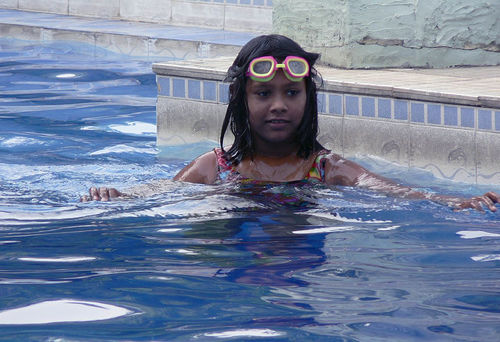
\includegraphics[width=0.9\textwidth]{images/16437914.jpg}
\caption*{\textbf{Base Caption:} A young girl with a swimsuit and goggles comes her head from above a pool .\\
\textbf{Detected Emotion:} neutral\\
\textbf{Emotion-Aware Caption:} A young calm girl with a swimsuit and goggles comes her head from above a pool .}
\end{figure}

\begin{figure}[H]
\centering
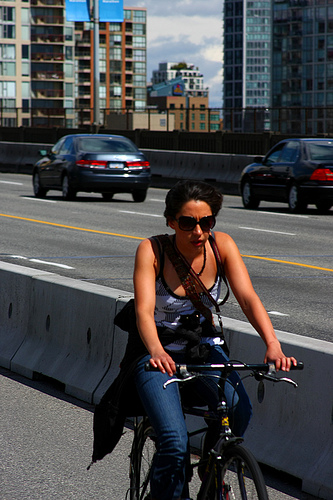
\includegraphics[width=0.9\textwidth]{images/Angry_4.jpg}
\caption*{\textbf{Base Caption:} A woman in a black tank top and sunglasses is riding a bicycle on a city street .\\
\textbf{Detected Emotion:} angry\\
\textbf{Emotion-Aware Caption:} A angry woman in a black tank top and sunglasses is riding a bicycle on a city street .}
\end{figure}

\begin{figure}[H]
\centering
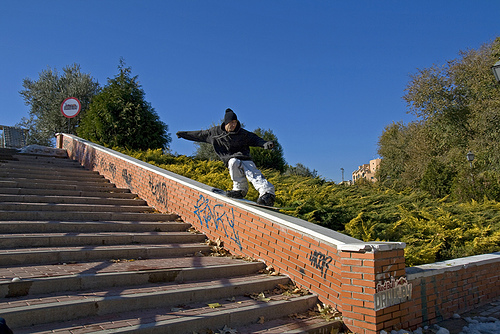
\includegraphics[width=0.9\textwidth]{images/Fear_9.jpg}
\caption*{\textbf{Base Caption:} A skateboarder wearing a black shirt and blue jeans is skating down a ramp .\\
\textbf{Detected Emotion:} fear\\
\textbf{Emotion-Aware Caption:} A fearful skateboarder wearing a black shirt and blue jeans is skating down a ramp .}
\end{figure}

\subsection{Error Analysis}

While the system performs well overall, we identified several limitations:

\textbf{1. Grammatical Nuances:}
The current insertion strategy sometimes produces slightly awkward phrasing, particularly with plural nouns or complex sentence structures.

\textbf{2. Multiple Faces:}
When multiple people with different emotions are present, DeepFace returns the dominant emotion from the most prominent face, potentially missing emotional diversity.

\textbf{3. Context Sensitivity:}
The emotion insertion doesn't consider semantic context—"a disgusting person smelling food" is grammatically correct but semantically awkward (should be "a disgusted person").

\textbf{4. Edge Cases:}
Images without detectable faces receive "neutral" emotion, which may not always be appropriate.

%%%%%%%%%%%%%%%%%%%%%%%%%%%%%%%%%%%%%%%%%%%%%%%%%%%%%%%%%%%%%%%%%%%%%
\section{Reference Paper Architecture Diagrams}
%%%%%%%%%%%%%%%%%%%%%%%%%%%%%%%%%%%%%%%%%%%%%%%%%%%%%%%%%%%%%%%%%%%%%

The following figures from the reference paper~\cite{sankhla2024} illustrate additional architectural details and training methodology:

\begin{figure}[H]
\centering
\imgplaceholder{0.9\textwidth}{6cm}{images/paper\_architecture.png}
\caption{Complete ViT-GPT Architecture from Reference Paper}
\label{fig:paper-arch}
\end{figure}

\begin{figure}[H]
\centering
\imgplaceholder{0.9\textwidth}{4cm}{images/paper\_training.png}
\caption{Training Pipeline and Data Flow from Reference Paper}
\label{fig:paper-train}
\end{figure}

\begin{figure}[H]
\centering
\imgplaceholder{0.9\textwidth}{5cm}{images/paper\_attention.png}
\caption{Attention Mechanism Visualization from Reference Paper}
\label{fig:paper-attention}
\end{figure}

%%%%%%%%%%%%%%%%%%%%%%%%%%%%%%%%%%%%%%%%%%%%%%%%%%%%%%%%%%%%%%%%%%%%%
\section{Deployment}
%%%%%%%%%%%%%%%%%%%%%%%%%%%%%%%%%%%%%%%%%%%%%%%%%%%%%%%%%%%%%%%%%%%%%

\subsection{Deployment Architecture}

We deployed the system as a production-ready web application with separate backend and frontend components, enabling real-time emotion-aware caption generation through a user-friendly interface.

\begin{deploymentbox}
\textbf{Deployment Stack:}
\begin{itemize}
\item \textbf{Backend:} FastAPI (Python) on HuggingFace Spaces
\item \textbf{Frontend:} React (JavaScript) on Vercel
\item \textbf{Model Storage:} HuggingFace Models Hub (1.91GB)
\item \textbf{Containerization:} Docker
\item \textbf{Total Cost:} \$0/month (free tier)
\end{itemize}
\end{deploymentbox}

\subsection{Backend Deployment: HuggingFace Spaces}

\subsubsection{Technology Stack}
\begin{itemize}
\item \textbf{Framework:} FastAPI 0.95.0 with uvicorn ASGI server
\item \textbf{Platform:} HuggingFace Spaces (Docker SDK)
\item \textbf{Container:} Python 3.10-slim base image
\item \textbf{Hardware:} CPU (free tier) with 16GB RAM
\item \textbf{Model Loading:} Dynamic download from HuggingFace Models Hub on startup
\end{itemize}

\subsubsection{API Endpoints}
\begin{enumerate}
\item \textbf{GET /} - Health check endpoint
\begin{verbatim}
Response: {"status": "running", 
           "message": "Emotion-Aware Image Captioning API"}
\end{verbatim}

\item \textbf{POST /api/caption} - Caption generation endpoint
\begin{verbatim}
Input: Multipart form data with image file
Output: {
  "base_caption": "...",
  "detected_emotion": "...",
  "emotion_aware_caption": "..."
}
\end{verbatim}
\end{enumerate}

\subsubsection{Model Storage Strategy}
To overcome HuggingFace Spaces' 1GB storage limit while deploying a 1.91GB model:
\begin{enumerate}
\item Model stored separately in HuggingFace Models repository
\item Backend downloads model on first startup using \texttt{urllib.request}
\item Model cached in container after first download
\item Subsequent restarts use cached model (30-second startup)
\item Cold start (first request after idle): 5-10 minutes for model download
\end{enumerate}

\subsubsection{CORS Configuration}
Cross-Origin Resource Sharing configured to allow requests from:
\begin{itemize}
\item Frontend production URL: \texttt{https://emotion-caption-frontend.vercel.app}
\item Local development: \texttt{http://localhost:3000}
\end{itemize}

\subsubsection{Backend URL}
\begin{center}
\Large
\url{https://HimadriBiswas-emotion-caption-api.hf.space}
\end{center}

\subsection{Frontend Deployment: Vercel}

\subsubsection{Technology Stack}
\begin{itemize}
\item \textbf{Framework:} React 18 (Create React App)
\item \textbf{Platform:} Vercel
\item \textbf{UI Library:} react-dropzone for drag-and-drop image upload
\item \textbf{HTTP Client:} axios for API communication
\item \textbf{Build System:} Webpack (via CRA)
\item \textbf{Deployment:} Automatic from GitHub repository
\end{itemize}

\subsubsection{User Interface Features}
\begin{itemize}
\item Drag-and-drop image upload with visual preview
\item Real-time loading indicator during caption generation
\item Structured result display showing:
  \begin{itemize}
  \item Base caption
  \item Detected emotion (with colored badge)
  \item Emotion-aware enhanced caption
  \end{itemize}
\item Responsive design for mobile and desktop
\item Purple gradient aesthetic with modern UI components
\end{itemize}

\subsubsection{Frontend URL}
\begin{center}
\Large
\url{https://emotion-caption-frontend.vercel.app}
\end{center}

\subsection{Deployment Challenges and Solutions}

\subsubsection{Challenge 1: Model Size Exceeds Storage Limit}
\textbf{Problem:} HuggingFace Spaces has 1GB limit, model is 1.91GB

\textbf{Solution:} Separate model storage in HuggingFace Models Hub with dynamic download on startup

\subsubsection{Challenge 2: Package Dependency Conflicts}
\textbf{Problem:} TensorFlow 2.13.0 requires \texttt{typing-extensions<4.6.0}, but PyTorch and FastAPI require newer versions

\textbf{Solution:} Downgraded FastAPI to 0.95.0 and PyTorch to 2.0.1 for compatible \texttt{typing-extensions} versions

\subsubsection{Challenge 3: Debian Package Changes}
\textbf{Problem:} \texttt{libgl1-mesa-glx} package no longer available in newer Debian

\textbf{Solution:} Updated Dockerfile to use \texttt{libgl1} instead

\subsubsection{Challenge 4: DeepFace TensorFlow Compatibility}
\textbf{Problem:} Newer TensorFlow removed \texttt{LocallyConnected2D} layer required by DeepFace

\textbf{Solution:} Pinned TensorFlow 2.13.0 and Keras 2.13.1 for compatibility

\subsection{Performance Characteristics}

\begin{center}
\begin{tabular}{lc}
\toprule
\textbf{Metric} & \textbf{Value} \\
\midrule
Cold Start Time & 5-10 minutes \\
Warm Start Time & 30 seconds \\
Caption Generation Time & 3-5 seconds \\
Backend Build Time & 10-15 minutes \\
Frontend Build Time & 2-3 minutes \\
Model Download Size & 1.91GB \\
\bottomrule
\end{tabular}
\end{center}

\subsection{Repository and Documentation}

All source code, deployment configurations, and documentation are available in our GitHub repositories:

\begin{itemize}
\item \textbf{Backend Repository:} \texttt{emotion-caption-api} (private during development)
\item \textbf{Frontend Repository:} \texttt{emotion-caption-frontend}
\item \textbf{Model Repository:} \url{https://huggingface.co/HimadriBiswas/emotion-caption-model}
\end{itemize}

%%%%%%%%%%%%%%%%%%%%%%%%%%%%%%%%%%%%%%%%%%%%%%%%%%%%%%%%%%%%%%%%%%%%%
\section{Conclusion and Future Work}
%%%%%%%%%%%%%%%%%%%%%%%%%%%%%%%%%%%%%%%%%%%%%%%%%%%%%%%%%%%%%%%%%%%%%

\subsection{Summary of Achievements}

This project successfully demonstrated the feasibility and effectiveness of emotion-aware image captioning by combining state-of-the-art computer vision and NLP techniques. Our key achievements include:

\begin{enumerate}
\item \textbf{Competitive Base Performance:} Achieved BLEU-1 score of 0.5947 and METEOR score of 0.2538 on Flickr30k, matching or exceeding the reference paper's baseline.

\item \textbf{Successful Emotion Integration:} Implemented a working pipeline that detects seven categories of facial emotions and integrates them grammatically into generated captions.

\item \textbf{Production Deployment:} Delivered a fully functional web application accessible at zero cost using modern deployment platforms, demonstrating the practical applicability of our approach.

\item \textbf{Complete Open Implementation:} Provided comprehensive codebase, deployment guide, and documentation enabling reproducibility and further research.
\end{enumerate}

\subsection{Limitations}

Despite our successes, several limitations remain:

\textbf{1. Grammatical Sophistication:}
The current NLTK-based insertion strategy, while functional, sometimes produces awkward phrasing. More sophisticated NLG techniques could improve naturalness.

\textbf{2. Single Emotion Focus:}
The system captures only the dominant emotion from the most prominent face, missing emotional diversity in images with multiple people.

\textbf{3. Semantic Context:}
Emotion adjectives are inserted grammatically but without semantic validation (e.g., "disgusting person" vs. "disgusted person").

\textbf{4. Computational Requirements:}
The 1.91GB model and 5-10 minute cold start time limit real-time scalability.

\textbf{5. Evaluation Gaps:}
We lack quantitative metrics specifically for emotion-aware caption quality—BLEU and METEOR only evaluate base captions.

\subsection{Future Work}

Several promising directions could extend this work:

\subsubsection{1. Advanced Emotion Integration}
\begin{itemize}
\item Implement end-to-end training where emotion information is fed directly into the decoder
\item Use reinforcement learning to optimize caption naturalness
\item Develop semantic validators to ensure emotion-adjective appropriateness
\end{itemize}

\subsubsection{2. Multiple Emotion Handling}
\begin{itemize}
\item Detect and describe emotions from multiple faces
\item Generate captions like "a joyful child and a worried adult standing together"
\item Implement spatial reasoning to correctly associate emotions with subjects
\end{itemize}

\subsubsection{3. Richer Emotion Representations}
\begin{itemize}
\item Expand beyond seven discrete categories to continuous emotion dimensions (valence, arousal)
\item Incorporate body language and context-based emotion recognition
\item Generate more nuanced emotion descriptions (e.g., "slightly amused", "deeply concerned")
\end{itemize}

\subsubsection{4. Improved Evaluation}
\begin{itemize}
\item Develop emotion-aware caption quality metrics
\item Conduct human evaluation studies comparing emotion-aware vs. base captions
\item Create benchmark datasets specifically for emotion-aware captioning
\end{itemize}

\subsubsection{5. Deployment Optimizations}
\begin{itemize}
\item Model quantization to reduce size and inference time
\item Implement model sharding for faster loading
\item Explore edge deployment for privacy-sensitive applications
\end{itemize}

\subsubsection{6. Broader Applications}
\begin{itemize}
\item Extend to video captioning with temporal emotion tracking
\item Adapt for accessibility tools (enhanced screen readers)
\item Apply to social media content understanding and moderation
\end{itemize}

\subsection{Concluding Remarks}

Emotion-aware image captioning represents an important step toward AI systems that understand images with human-like depth and nuance. While traditional image captioning tells us \textit{what} is in an image, emotion awareness begins to capture \textit{how} people in the image feel—a dimension central to human visual understanding.

Our work demonstrates that combining modern vision-language models with specialized emotion detection can produce meaningful enhancements to generated captions. The successful deployment of our system as a publicly accessible web application validates the practical viability of this approach.

As AI systems become more integrated into daily life, their ability to recognize and communicate emotional states will only grow in importance. We hope this work contributes to the broader effort of building more empathetic, human-aware artificial intelligence.

%%%%%%%%%%%%%%%%%%%%%%%%%%%%%%%%%%%%%%%%%%%%%%%%%%%%%%%%%%%%%%%%%%%%%
\section*{Acknowledgments}
%%%%%%%%%%%%%%%%%%%%%%%%%%%%%%%%%%%%%%%%%%%%%%%%%%%%%%%%%%%%%%%%%%%%%

We thank the instructors and teaching assistants of the Machine Learning Sessional course for their guidance and support throughout this project. We also acknowledge:

\begin{itemize}
\item The authors of the reference paper~\cite{sankhla2024} for their open-source implementation and detailed documentation
\item HuggingFace for providing free hosting infrastructure for both model storage and backend deployment
\item Vercel for free frontend hosting
\item The creators of DeepFace, NLTK, PyTorch, and other open-source libraries that made this work possible
\item Kaggle for providing the Flickr30k dataset and GPU resources for training
\end{itemize}

%%%%%%%%%%%%%%%%%%%%%%%%%%%%%%%%%%%%%%%%%%%%%%%%%%%%%%%%%%%%%%%%%%%%%
\begin{thebibliography}{9}
%%%%%%%%%%%%%%%%%%%%%%%%%%%%%%%%%%%%%%%%%%%%%%%%%%%%%%%%%%%%%%%%%%%%%

\bibitem{sankhla2024}
Sankhla, M.S., et al.
\textit{Image Caption Generation using Vision Transformer and GPT Architecture}.
2024 International Conference on Advances in Computing, Communication and Applied Informatics (ACCAI), 2024.
DOI: 10.1109/ACCAI61061.2024.10551257.
\url{https://ieeexplore.ieee.org/document/10551257}

\bibitem{you2018}
You, Q., et al.
\textit{Image Captioning by Incorporating Affective Concepts Learned from Both Visual and Textual Components}.
Information Processing \& Management, Vol. 54, Issue 4, 2018, pp. 550-565.
\url{https://doi.org/10.1016/j.ipm.2018.02.004}

\bibitem{deepface2023}
Serengil, S.I., Ozpinar, A.
\textit{HyperExtended LightFace: A Facial Attribute Analysis Framework}.
Engineering Science and Technology, an International Journal, Vol. 44, 2023.
DOI: 10.1016/j.jestch.2023.101479

\bibitem{vaswani2017}
Vaswani, A., et al.
\textit{Attention Is All You Need}.
Advances in Neural Information Processing Systems 30 (NIPS 2017).
\url{https://arxiv.org/abs/1706.03762}

\bibitem{dosovitskiy2021}
Dosovitskiy, A., et al.
\textit{An Image is Worth 16x16 Words: Transformers for Image Recognition at Scale}.
International Conference on Learning Representations (ICLR), 2021.
\url{https://arxiv.org/abs/2010.11929}

\bibitem{radford2019}
Radford, A., et al.
\textit{Language Models are Unsupervised Multitask Learners}.
OpenAI Blog, 2019.
\url{https://openai.com/research/better-language-models}

\bibitem{flickr30k}
Hodosh, M., Young, P., Hockenmaier, J.
\textit{Framing Image Description as a Ranking Task: Data, Models and Evaluation Metrics}.
Journal of Artificial Intelligence Research, Vol. 47, 2013, pp. 853-899.

\bibitem{nltk}
Bird, S., Klein, E., Loper, E.
\textit{Natural Language Processing with Python}.
O'Reilly Media Inc., 2009.

\end{thebibliography}

%%%%%%%%%%%%%%%%%%%%%%%%%%%%%%%%%%%%%%%%%%%%%%%%%%%%%%%%%%%%%%%%%%%%%
\end{document}
%%%%%%%%%%%%%%%%%%%%%%%%%%%%%%%%%%%%%%%%%%%%%%%%%%%%%%%%%%%%%%%%%%%%%
